%% abtex2-modelo-relatorio-tecnico.tex, v-1.7.1 laurocesar
%% Copyright 2012-2013 by abnTeX2 group at http://abntex2.googlecode.com/ 
%%
%% This work may be distributed and/or modified under the
%% conditions of the LaTeX Project Public License, either version 1.3
%% of this license or (at your option) any later version.
%% The latest version of this license is in
%%   http://www.latex-project.org/lppl.txt
%% and version 1.3 or later is part of all distributions of LaTeX
%% version 2005/12/01 or later.
%%
%% This work has the LPPL maintenance status `maintained'.
%% 
%% The Current Maintainer of this work is the abnTeX2 team, led
%% by Lauro César Araujo. Further information are available on 
%% http://abntex2.googlecode.com/
%%
%% This work consists of the files abntex2-modelo-relatorio-tecnico.tex,
%% abntex2-modelo-include-comandos and abntex2-modelo-references.bib
%%

% ------------------------------------------------------------------------
% ------------------------------------------------------------------------
% abnTeX2: Modelo de Relatório Técnico/Acadêmico em conformidade com 
% ABNT NBR 10719:2011 Informação e documentação - Relatório técnico e/ou
% científico - Apresentação
% ------------------------------------------------------------------------ 
% ------------------------------------------------------------------------

% Alterado por Rodrigo Campiolo para apresentação de relatórios na disciplina
% de Redes de Computadores II do Bacharelado em Ciência da Computação da UTFPR-CM.


\documentclass[
	% -- opções da classe memoir --
	12pt,				% tamanho da fonte
	%openright,			% capítulos começam em pág ímpar (insere página vazia caso preciso)
	oneside,   	        % para impressão em verso e anverso use twoside. Oposto a oneside
	a4paper,			% tamanho do papel. 
	% -- opções da classe abntex2 --
	%chapter=TITLE,		% títulos de capítulos convertidos em letras maiúsculas
	%section=TITLE,		% títulos de seções convertidos em letras maiúsculas
	%subsection=TITLE,	% títulos de subseções convertidos em letras maiúsculas
	%subsubsection=TITLE,% títulos de subsubseções convertidos em letras maiúsculas
	% -- opções do pacote babel --
	english,			% idioma adicional para hifenização
	french,				% idioma adicional para hifenização
	spanish,			% idioma adicional para hifenização
	brazil,				% o último idioma é o principal do documento
	]{pacotes/abntex2}


% ---
% PACOTES
% ---

% ---
% Pacotes fundamentais 
% ---
\usepackage{cmap}				% Mapear caracteres especiais no PDF
\usepackage{lmodern}			% Usa a fonte Latin Modern
\usepackage[T1]{fontenc}		% Selecao de codigos de fonte.
\usepackage[utf8]{inputenc}		% Codificacao do documento (conversão automática dos acentos)
\usepackage{indentfirst}		% Indenta o primeiro parágrafo de cada seção.
\usepackage{color}				% Controle das cores
\usepackage{graphicx}			% Inclusão de gráficos
% ---

% ---
% Pacotes adicionais, usados no anexo do modelo de folha de identificação
% ---
\usepackage{multicol}
\usepackage{multirow}
% ---
	
% ---
% Pacotes adicionais, usados apenas no âmbito do Modelo Canônico do abnteX2
% ---
\usepackage{lipsum}				% para geração de dummy text
% ---

% ---
% Pacotes de citações
% ---
\usepackage[brazilian,hyperpageref]{backref}	 % Paginas com as citações na bibl
\usepackage[alf]{pacotes/abntex2cite}	% Citações padrão ABNT
\usepackage{comment}
% ---

% ---
% Meus pacotes
% ---
\usepackage{float}
\usepackage{array}
% ---

% --- 
% CONFIGURAÇÕES DE PACOTES
% --- 

% ---
% Configurações do pacote backref
% Usado sem a opção hyperpageref de backref
\renewcommand{\backrefpagesname}{Citado na(s) página(s):~}
% Texto padrão antes do número das páginas
\renewcommand{\backref}{}
% Define os textos da citação
\renewcommand*{\backrefalt}[4]{
	\ifcase #1 %
		Nenhuma citação no texto.%
	\or
		Citado na página #2.%
	\else
		Citado #1 vezes nas páginas #2.%
	\fi}%
% ---

% ---
% Informações de dados para CAPA e FOLHA DE ROSTO
% ---
\titulo{Manipulação de \textit{Threads}}
\autor{Hendrick Felipe Scheifer\\João Victor Briganti\\Luiz Gustavo Takeda}
\local{Campo Mourão}
\data{Outubro / 2024}
\instituicao{%
  Universidade Tecnológica Federal do Paraná -- UTFPR
  \par
  Departa           mento Acadêmico de Computação -- DACOM
  \par
  Bacharelado em Ciência da Computação -- BCC
}
\tipotrabalho{Relatório técnico}
% O preambulo deve conter o tipo do trabalho, o objetivo, 
% o nome da instituição e a área de concentração 
\preambulo{Relatório técnico de atividade prática solicitado pelo professor Rodrigo Campiolo na disciplina de Sistemas Operacionais do Bacharelado em Ciência da Computação da Universidade Tecnológica Federal do Paraná.}
% ---

% ---
% Configurações de aparência do PDF final

% alterando o aspecto da cor azul
\definecolor{blue}{RGB}{41,5,195}

% informações do PDF
\makeatletter
\hypersetup{
     	%pagebackref=true,
		pdftitle={\@title}, 
		pdfauthor={\@author},
    	pdfsubject={\imprimirpreambulo},
	    pdfcreator={LaTeX with abnTeX2},
		pdfkeywords={abnt}{latex}{abntex}{abntex2}{relatório técnico}, 
		colorlinks=true,       		% false: boxed links; true: colored links
    	linkcolor=blue,          	% color of internal links
    	citecolor=blue,        		% color of links to bibliography
    	filecolor=magenta,      		% color of file links
		urlcolor=blue,
		bookmarksdepth=4
}
\makeatother
% --- 

% --- 
% Espaçamentos entre linhas e parágrafos 
% --- 

% O tamanho do parágrafo é dado por:
\setlength{\parindent}{1.3cm}

% Controle do espaçamento entre um parágrafo e outro:
\setlength{\parskip}{0.2cm}  % tente também \onelineskip

% ---
% compila o indice
% ---
\makeindex
% ---

% Omite a numeração de capítulos
\renewcommand*\thesection{\arabic{section}}



% ----
% Início do documento
% ----
\begin{document}

% Retira espaço extra obsoleto entre as frases.
\frenchspacing 

% ----------------------------------------------------------
% ELEMENTOS PRÉ-TEXTUAIS
% ----------------------------------------------------------
% \pretextual

% ---
% Capa
% ---
%\imprimircapa
% ---

% ---
% Folha de rosto
% (o * indica que haverá a ficha bibliográfica)
% ---
\imprimirfolhaderosto
% ---


% ---
% RESUMO
% ---

% resumo na língua vernácula (obrigatório)
\begin{resumo}
Este trabalho visa aplicar conceitos práticos sobre operações com \textit{threads}, explorando o uso da biblioteca \textit{pthreadsto} para a criação de programas. Utiliando o hipervisor VirtualBox versão 7.1.2 para configurar uma máquina virtual com o sistema operacional GNU/Linux Debian. Os procedimentos realizados foram a listagem das \textit{threads} em execução, verificação do número máximo de \textit{threads} que o sistema suporta e a medição do tempo de execução de um programa que realiza cálculos de matrizes. Os resultados foram satisfatórios, alcançando os objetivos propostos e proporcionando uma melhor compreensão sobre a utilização de \textit{threads} na programação.

 \vspace{\onelineskip}
    
 \noindent
 \textbf{Palavras-chave}: VirtualBox. Debian. Sistema Operacional.
\end{resumo}
% ---

% ---
% inserir lista de ilustrações
% ---
%\pdfbookmark[0]{\listfigurename}{lof}
%\listoffigures*
%\cleardoublepage
% ---

% ---
% inserir lista de tabelas
% ---
%\pdfbookmark[0]{\listtablename}{lot}
%\listoftables*
%\cleardoublepage
% ---

% ---
% inserir lista de abreviaturas e siglas
% ---
%\begin{siglas}
%  \item[IP] Internet Protocol
%  \item[TCP] Transmission Control Protocol
%  \item[UDP] User Datagram Protocol
%\end{siglas}
% ---

% ---
% inserir o sumario
% ---
\pdfbookmark[0]{\contentsname}{toc}
\tableofcontents*
\cleardoublepage
% ---

% ----------------------------------------------------------
% ELEMENTOS TEXTUAIS
% ----------------------------------------------------------
\textual

\makeatletter
\renewcommand{\chapter}{\@gobbletwo}
\makeatother

\section{Introdução}
\label{sec:introducao}
A princípio, os sistemas operacionais não suportavam mais de uma tarefa por processo, o que se tornou um grande problema conforme a complexidade das aplicações desenvolvidas se tornou maior. Uma mesma aplicação atualmente exerce diversas funções simultâneas, o que gerou a necessidade de mais de uma tarefa em um mesmo processo, operando sob os mesmos recursos~\cite{maziero2019}.

Para resolver o problema citado anteriormente, surgem fluxos de execuções independentes menores em um mesmo processo, denominados \textit{threads}, que compartilham recursos umas com as outras~\cite{maziero2019}. Tais \textit{threads} são essenciais em aplicações que exigem que diversas funções sejam executadas simultaneamente, e são muito mais leves, tornado-as mais rápidas para criar e destruir, além de favorecerem o desempenho das aplicações, visto que torna a computação e entradas/saídas substanciais, permitindo a sobreposição destas atividades~\cite{tanenbaum2016}. 

\section{Objetivos}
\label{sec:objetivos}

Este trabalho tem como objetivo explorar e detalhar a criação e manipulação de \textit{threads} em um ambiente GNU/Linux, fornecendo explicações abrangentes sobre a biblioteca utilizada para essa manipulação.

\section{Fundamentação}
\label{sec:fundamentacao}
\textit{Threads} de núcleo são utilizadas para mapear \textit{threads} de usuário dentro do núcleo do sistema operacional. Além de serem utilizadas por atividades internas do próprio núcleo. A forma como as \textit{threads} de usuário serão mapeadas para as de núcleo dependem do modelo de implementação utilizado~\cite{maziero2019}.

Os principais modelos de \textit{threads} são os seguintes modelos: N:1, onde várias \textit{threads} de usuários são mapeadas para uma \textit{thread} de núcleo, reduzindo a carga de gerência, visto que o núcleo enxerga tudo como uma única \textit{thread}. Temos também o modelo 1:1, onde cada \textit{thread} de  usuário gera uma de núcleo, tornando a distribuição do processamento entre \textit{threads} mais justa, porém é pouco escalável devido à grande carga de \textit{threads} de núcleo geradas em aplicações maiores. E por fim temos o modelo N:M, que é uma abordagem híbrida entre os dois modelos citados anteriormente, onde N \textit{thread} de usuário são mapeadas para M \textit{threads} de núcleo (sendo M<N), esta abordagem, embora mais complexa, explora o melhor de cada um dos outros dois modelos~\cite{maziero2019}.

Antes de 1995, cada sistema operacional criava sua própria interface para a programação de \textit{threads}. Mas no ano citado, foi estabelecido o padrão \textit{IEEE POSIX 1003.1c}, popularmente conhecido como \textit{POSIX Threads}, e abreviado ainda para \textit{PThreads}, este padrão determina uma interface para a utilização de \textit{threads} na linguagem C e ainda é amplamente suportado e disseminado atualmente~\cite{maziero2019}.

\section{Materiais e Equipamentos}
\label{sec:materiais}

\begin{itemize}
  \item Especificações do computador utilizado:
  \begin{itemize}
    \item Modelo: Notebook Lenovo Thinkpad E14
    \item CPU: AMD Ryzen $5$-$3500$U
    \item Memória Principal: $8$\,GB RAM
    \item Memória Secundária: SSD $256$\,GB NVMe
    \item Sistema Operacional: Fedora $40$
  \end{itemize}
  \item Hipervisor: VirtualBox $7.1.2$
  \item Sistema Operacional no Hipervisor: GNU/Linux Debian $12.7$
  \item Núcleo: Linux $6.10.11$
\end{itemize}

\section{Procedimentos e Resultados}
\label{sec:procedimentos}

Nesta seção, apresentaremos os procedimentos utilizados para a manipulação de \textit{threads} em um ambiente GNU/Linux. Abordaremos a verificação do número de \textit{threads} em execução, a capacidade máxima suportada e o impacto no desempenho de programas gerados por essas \textit{threads}.

\subsection{Listagem de \textit{Threads}}
\label{subsec:list_threads}

No sistema GNU/Linux, é possível obter informações sobre o estado do sistema através da leitura de arquivos localizados em \texttt{/proc}~\cite{negus2012}. Na Figura~\ref{fig:total_tid}, apresentamos a leitura do arquivo \texttt{/proc/loadavg}, que fornece dados sobre a carga média de execução do sistema. Na quarta coluna, após o símbolo ``/'', verificamos que o sistema possui 115 \textit{threads} em execução.

\begin{figure}[H]
  \centering
  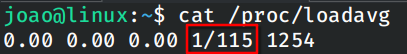
\includegraphics[scale=0.45]{figuras/total_tid.png}
  \caption{Saída da leitura do arquivo \texttt{/proc/loadavg}.}
  \label{fig:total_tid}
\end{figure}

A listagem das \textit{threads} pode ser realizada com a execução do seguinte comando \texttt{ps -eLo pid,lwp,nlwp,user,cmd --sort -nlwp}, cuja saída é apresentada na Figura~\ref{fig:ps}.

\begin{figure}[H]
  \centering
  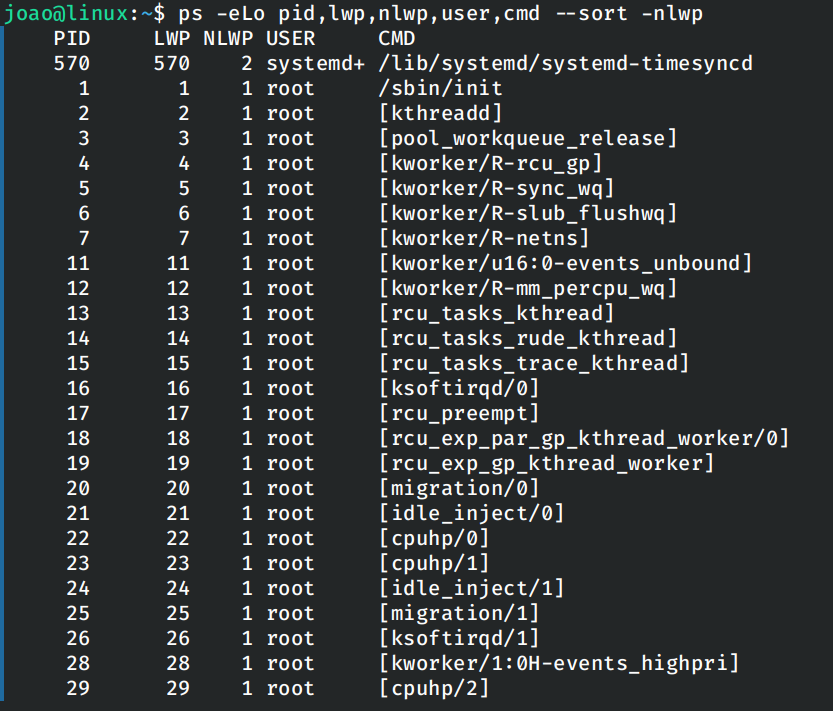
\includegraphics[scale=0.45]{figuras/ps.png}
  \caption{Saída do comando \texttt{ps -eLo pid,lwp,nlwp,user,cmd --sort -nlwp}.}
  \label{fig:ps}
\end{figure}

O comando \textit{ps} utilizado para a visualização das \textit{threads} apresenta as seguintes \textit{flags}~\cite{shotts2017}:

\begin{itemize}
    \item \textbf{e:} Seleciona todos os processos.
    \item \textbf{o:} Permite ao usuário definir o formato da saída. No comando, foram selecionadas as seguintes informações:
    \begin{itemize}
        \item \textbf{pid:} ID do processo.
        \item \textbf{lwp:} ID da \textit{thread}.
        \item \textbf{nlwp:} Número de \textit{threads} associadas a este processo.
        \item \textbf{user:} Nome do usuário proprietário do processo em execução.
        \item \textbf{cmd:} Comando que está sendo executado.
    \end{itemize}
    \item \textbf{sort:} Ordena a saída de forma decrescente com base no número de \textit{threads}, conforme especificado pela \textit{-nlwp}.
\end{itemize}

Na saída apresentada na Figura~\ref{fig:ps}, o processo com o maior número de \textit{threads} é o comando \texttt{/lib/systemd/systemd-timesyncd}, que possui um total de 2 \textit{threads}. Os demais processos listados têm apenas 1 \textit{thread} cada.

\subsection{Número Máximo de \textit{Threads}}
\label{subsec:max_threads}

Informações sobre o número máximo de \textit{threads} que podem ser criadas no sistema também podem ser obtidas através da leitura de arquivos em \texttt{/proc}~\cite{negus2012}. Na Figura~\ref{fig:max_threads}, apresentamos a leitura do arquivo \texttt{/proc/sys/kernel/max\_threads}, que exibe o número máximo permitido de \textit{threads}.

\begin{figure}[H]
  \centering
  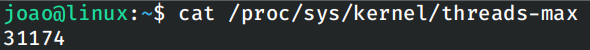
\includegraphics[scale=0.45]{figuras/max_threads.png}
  \caption{Saída da leitura do arquivo \texttt{/proc/sys/kernel/max\_threads}.}
  \label{fig:max_threads}
\end{figure}

\subsection{Tempo de Execução}
\label{subsec:time}

Utilizando a biblioteca \textit{pthread}, foi desenvolvido um programa para calcular, de maneira paralela, a média aritmética das linhas e a média geométrica das colunas de uma matriz $M \times N$. Os resultados são salvos em um arquivo de texto especificado pelo usuário.

Esta implementação adota técnicas de paralelização de funções e dados, distribuindo as tarefas de cálculo entre várias threads para maximizar a eficiência do processamento.

As especificações do sistema que executou o programa, estão detalhadas na Seção~\ref{sec:materiais}, e a matriz de entrada possui o tamanho $100 \times 200$. A Tabela~\ref{table:time} mostra o tempo de execução do programa com 1, 2, 4, 8 e 16 \textit{threads}, destacando o impacto da paralelização.

\begin{table}[!htb]
\centering
\caption{Tempo de execução para diferentes quantidades de \textit{threads}}
\label{table:time}
\footnotesize
\begin{tabular}{@{}l|lll@{}}
\toprule
\textbf{Número de \textit{threads}} & \textbf{Tempo Real (ms)} & \textbf{Tempo de Sistema (ms)} & \textbf{Tempo de Usuário (ms)}\\ 
\midrule
1 & 24 & 8 & 7 \\
2 & 24 & 11 & 4 \\
4 & 20 & 15 & 15 \\
8 & 20 & 13 & 20 \\
16 & 21 & 13 & 15 \\
\bottomrule
\end{tabular}
\end{table}

Para cada execução, foram medidos três tipos de tempo:

\begin{itemize}
    \item \textbf{Tempo Real:} Representa o tempo total decorrido durante a execução.
    \item \textbf{Tempo de Sistema:} Indica o tempo gasto de execução operações do núcleo.
    \item \textbf{Tempo de Usuário:} Indica o tempo dedicado à execução do código de usuário do programa.
\end{itemize}

Os resultados mostram que o tempo real permaneceu estável, em torno de 20 ms, independentemente do número de \textit{threads}. O tempo de sistema variou, com a execução em uma única \textit{thread} apresentando um tempo menor em relação às demais, enquanto nas execuções com múltiplas \textit{threads}, o tempo aumentou ligeiramente, atingindo valores entre 11 e 15 ms. Por outro lado, o tempo de usuário foi menor para a execução com 2 \textit{threads}, atingindo um tempo médio de 4 ms, em comparação com as execuções com 4 \textit{threads} ou mais, nas quais variou entre 13 e 20 ms.

\section{Discussão dos Resultados}
\label{sec:discussao}
FAZER

\section{Conclusões}
\label{sec:conclusoes}
FAZER

% ----------------------------------------------------------
% ELEMENTOS PÓS-TEXTUAIS
% ----------------------------------------------------------
\postextual
% ----------------------------------------------------------
% Referências bibliográficas
% ----------------------------------------------------------
\renewcommand{\bibsection}{%
\section{\bibname}
\bibmark
%\ifnobibintoc\else
%\phantomsection
%\addcontentsline{toc}{section}{\bibname}
%\fi
\prebibhook}

\bibliography{abntex2-modelo-references}

\end{document}
